% Coarsest G2 Grassmannian cell 29: rays 13,14,17,18, with its rays clockwise from the top left corner; G2-trees, generated by julia/to_tex/square_cell_figure.jl
\begingroup
\definecolor{g2RayLabel}{HTML}{000000}
\definecolor{g2CellLabel}{HTML}{000000}
\definecolor{g2TaxonBlue}{HTML}{1676A3}
\colorlet{g2SquareFill}{g2TaxonBlue!10}
\tikzset{
  g2square side/.style={draw=g2RayLabel,line width=.8pt},
  g2square circle/.style={draw=g2RayLabel,fill=white,line width=.8pt},
  g2square cell/.style={fill=g2SquareFill},
  g2square name/.style={text=g2RayLabel,inner sep=0pt,font=\boldmath},
  g2square cell name/.style={g2square name,text=g2CellLabel},
}
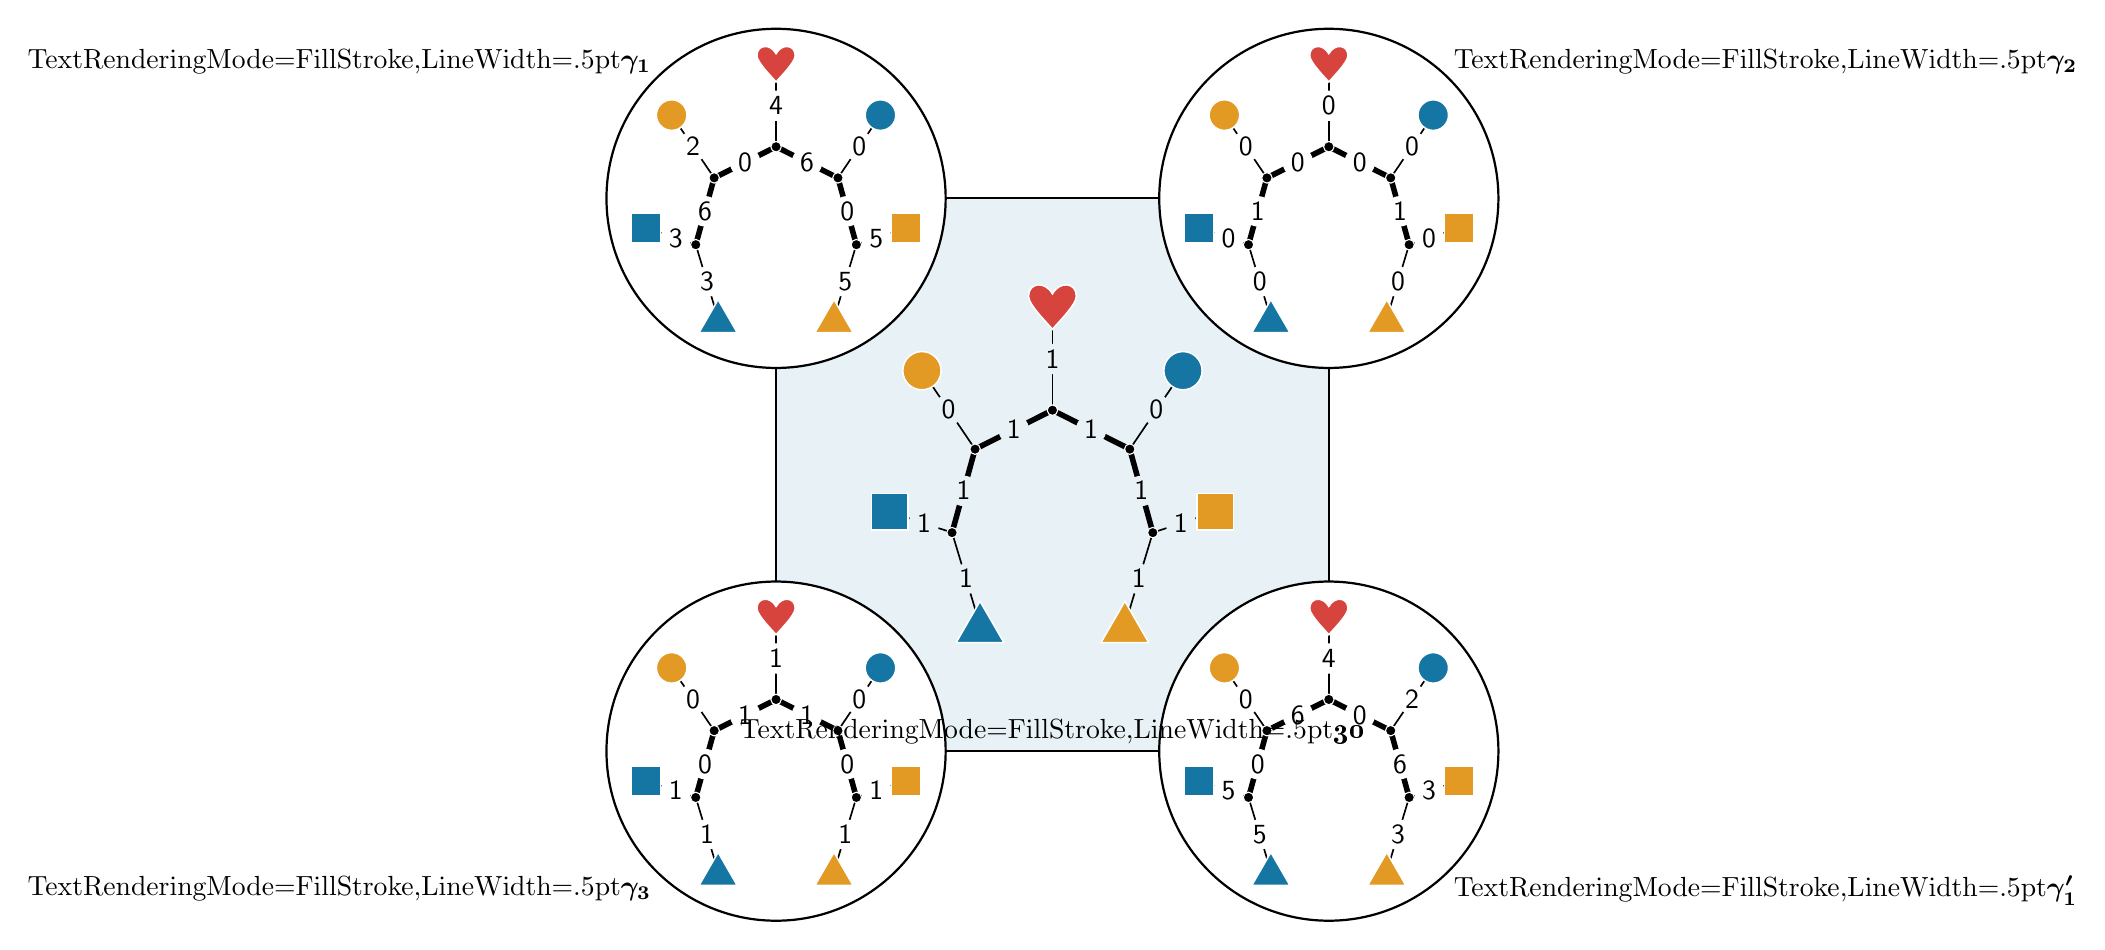
\begin{tikzpicture}[x=1cm,y=1cm,baseline=(current bounding box.center)]
\fill[g2square cell] (-3.51,3.51)--(3.51,3.51)--(3.51,-3.51)--(-3.51,-3.51)--cycle;
\draw[g2square side] (-3.51,3.51)--(3.51,3.51)--(3.51,-3.51)--(-3.51,-3.51)--cycle;
% Ray 13
\draw[g2square circle] (-3.51,3.51) circle[radius=2.1538];
\node[g2square name,anchor=south east] at (-5.0895,5.0895) {\textpdfrender{TextRenderingMode=FillStroke,LineWidth=.5pt}{\bfseries\boldmath \(\gamma_1\)}};
\begin{scope}[shift={(-3.51,3.51)}]
\begingroup
\definecolor{g2TaxonBlue}{HTML}{1676A3}
\definecolor{g2TaxonYellow}{HTML}{E39A24}
\definecolor{g2HeartRed}{HTML}{D7443E}
\tikzset{
  g2tree pendant/.style={draw=black,line width=.6pt,line cap=round},
  g2tree internal/.style={draw=black,line width=2pt,line cap=round},
  g2tree vertex/.style={circle,fill=black,draw=white,line width=.4pt,inner sep=0pt,minimum size=3.8pt},
  g2tree dark/.style={fill=g2TaxonBlue,draw=white,line width=.55pt,text=white,inner sep=0pt},
  g2tree light/.style={fill=g2TaxonYellow,draw=white,line width=.55pt,text=white,inner sep=0pt},
  g2tree weight/.style={circle,fill=white,draw=none,text=black,inner sep=.15pt,minimum size=8.5pt},
  g2tree aligned pendant/.style={fill=white,text=black,inner sep=.7pt,sloped,above=1pt,font={\sffamily\fontsize{7.5}{8}\selectfont}},
  g2tree aligned internal/.style={fill=white,text=black,inner sep=1pt,sloped,above=1pt,font={\sffamily\fontsize{7.5}{8}\selectfont\bfseries}},
}
\tikzset{g2tree weight/.append style={minimum size=11.0pt}}
\coordinate (v1) at (-1.65348,-0.37740);
\coordinate (v2) at (-0.73587,-1.52804);
\coordinate (v3) at (1.32599,1.05744);
\coordinate (v4) at (1.65348,-0.37740);
\coordinate (v5) at (0.73587,-1.52804);
\coordinate (v6) at (-1.32599,1.05744);
\coordinate (v7) at (0.00000,1.69600);
\coordinate (v8) at (-1.01986,-0.58816);
\coordinate (v9) at (1.01986,-0.58816);
\coordinate (v10) at (0.78600,0.26020);
\coordinate (v11) at (-0.78600,0.26020);
\coordinate (v12) at (-0.00000,0.65593);
\draw[g2tree internal] (v8)--(v11);
\draw[g2tree internal] (v9)--(v10);
\draw[g2tree internal] (v10)--(v12);
\draw[g2tree internal] (v11)--(v12);
\draw[g2tree pendant] (v1)--(v8);
\draw[g2tree pendant] (v2)--(v8);
\draw[g2tree pendant] (v3)--(v10);
\draw[g2tree pendant] (v4)--(v9);
\draw[g2tree pendant] (v5)--(v9);
\draw[g2tree pendant] (v6)--(v11);
\draw[g2tree pendant] (v7)--(v12);
\node[g2tree weight,font={\sffamily\fontsize{10}{10.5}\selectfont}] at (-0.90293,-0.16398) {6};
\node[g2tree weight,font={\sffamily\fontsize{10}{10.5}\selectfont}] at (0.90293,-0.16398) {0};
\node[g2tree weight,font={\sffamily\fontsize{10}{10.5}\selectfont}] at (0.39300,0.45806) {6};
\node[g2tree weight,font={\sffamily\fontsize{10}{10.5}\selectfont}] at (-0.39300,0.45806) {0};
\node[g2tree weight,font={\sffamily\fontsize{10}{10.5}\selectfont}] at (-1.27331,-0.50385) {3};
\node[g2tree weight,font={\sffamily\fontsize{10}{10.5}\selectfont}] at (-0.87786,-1.05810) {3};
\node[g2tree weight,font={\sffamily\fontsize{10}{10.5}\selectfont}] at (1.05599,0.65882) {0};
\node[g2tree weight,font={\sffamily\fontsize{10}{10.5}\selectfont}] at (1.27331,-0.50385) {5};
\node[g2tree weight,font={\sffamily\fontsize{10}{10.5}\selectfont}] at (0.87786,-1.05810) {5};
\node[g2tree weight,font={\sffamily\fontsize{10}{10.5}\selectfont}] at (-1.05599,0.65882) {2};
\node[g2tree weight,font={\sffamily\fontsize{10}{10.5}\selectfont}] at (0.00000,1.17597) {4};
\node[g2tree vertex] at (v8) {};
\node[g2tree vertex] at (v9) {};
\node[g2tree vertex] at (v10) {};
\node[g2tree vertex] at (v11) {};
\node[g2tree vertex] at (v12) {};
\node[g2tree dark,rectangle,minimum size=3.7260000000000004mm,font={\sffamily\fontsize{7.2}{7.2}\selectfont\bfseries}] at (v1) {};
\begin{scope}[shift={(v2)},scale=0.8100000000000002,transform shape]
\path[fill=g2TaxonBlue,draw=white,line width=.55pt,line join=round] (0mm,3.0mm)--(-3.0mm,-2.2mm)--(3.0mm,-2.2mm)--cycle;
\end{scope}
\node[g2tree dark,circle,minimum size=3.888000000000001mm,font={\sffamily\fontsize{7.2}{7.2}\selectfont\bfseries}] at (v3) {};
\node[g2tree light,rectangle,minimum size=3.7260000000000004mm,font={\sffamily\fontsize{7.2}{7.2}\selectfont\bfseries}] at (v4) {};
\begin{scope}[shift={(v5)},scale=0.8100000000000002,transform shape]
\path[fill=g2TaxonYellow,draw=white,line width=.55pt,line join=round] (0mm,3.0mm)--(-3.0mm,-2.2mm)--(3.0mm,-2.2mm)--cycle;
\end{scope}
\node[g2tree light,circle,minimum size=3.888000000000001mm,font={\sffamily\fontsize{7.2}{7.2}\selectfont\bfseries}] at (v6) {};
\begin{scope}[shift={(v7)},scale=0.8100000000000002,transform shape]
\path[fill=g2HeartRed,draw=white,line width=.55pt]
  (0mm,-2.7mm)..controls(-.45mm,-2.1mm)and(-3.0mm,.35mm)..(-3.0mm,1.45mm)
  ..controls(-3.0mm,3.2mm)and(-.9mm,3.4mm)..(0mm,1.75mm)
  ..controls(.9mm,3.4mm)and(3.0mm,3.2mm)..(3.0mm,1.45mm)
  ..controls(3.0mm,.35mm)and(.45mm,-2.1mm)..(0mm,-2.7mm)--cycle;
\end{scope}
\endgroup
\end{scope}
% Ray 14
\draw[g2square circle] (3.51,3.51) circle[radius=2.1538];
\node[g2square name,anchor=south west] at (5.0895,5.0895) {\textpdfrender{TextRenderingMode=FillStroke,LineWidth=.5pt}{\bfseries\boldmath \(\gamma_2\)}};
\begin{scope}[shift={(3.51,3.51)}]
\begingroup
\definecolor{g2TaxonBlue}{HTML}{1676A3}
\definecolor{g2TaxonYellow}{HTML}{E39A24}
\definecolor{g2HeartRed}{HTML}{D7443E}
\tikzset{
  g2tree pendant/.style={draw=black,line width=.6pt,line cap=round},
  g2tree internal/.style={draw=black,line width=2pt,line cap=round},
  g2tree vertex/.style={circle,fill=black,draw=white,line width=.4pt,inner sep=0pt,minimum size=3.8pt},
  g2tree dark/.style={fill=g2TaxonBlue,draw=white,line width=.55pt,text=white,inner sep=0pt},
  g2tree light/.style={fill=g2TaxonYellow,draw=white,line width=.55pt,text=white,inner sep=0pt},
  g2tree weight/.style={circle,fill=white,draw=none,text=black,inner sep=.15pt,minimum size=8.5pt},
  g2tree aligned pendant/.style={fill=white,text=black,inner sep=.7pt,sloped,above=1pt,font={\sffamily\fontsize{7.5}{8}\selectfont}},
  g2tree aligned internal/.style={fill=white,text=black,inner sep=1pt,sloped,above=1pt,font={\sffamily\fontsize{7.5}{8}\selectfont\bfseries}},
}
\tikzset{g2tree weight/.append style={minimum size=11.0pt}}
\coordinate (v1) at (-1.65348,-0.37740);
\coordinate (v2) at (-0.73587,-1.52804);
\coordinate (v3) at (1.32599,1.05744);
\coordinate (v4) at (1.65348,-0.37740);
\coordinate (v5) at (0.73587,-1.52804);
\coordinate (v6) at (-1.32599,1.05744);
\coordinate (v7) at (0.00000,1.69600);
\coordinate (v8) at (-1.01986,-0.58816);
\coordinate (v9) at (1.01986,-0.58816);
\coordinate (v10) at (0.78600,0.26020);
\coordinate (v11) at (-0.78600,0.26020);
\coordinate (v12) at (-0.00000,0.65593);
\draw[g2tree internal] (v8)--(v11);
\draw[g2tree internal] (v9)--(v10);
\draw[g2tree internal] (v10)--(v12);
\draw[g2tree internal] (v11)--(v12);
\draw[g2tree pendant] (v1)--(v8);
\draw[g2tree pendant] (v2)--(v8);
\draw[g2tree pendant] (v3)--(v10);
\draw[g2tree pendant] (v4)--(v9);
\draw[g2tree pendant] (v5)--(v9);
\draw[g2tree pendant] (v6)--(v11);
\draw[g2tree pendant] (v7)--(v12);
\node[g2tree weight,font={\sffamily\fontsize{10}{10.5}\selectfont}] at (-0.90293,-0.16398) {1};
\node[g2tree weight,font={\sffamily\fontsize{10}{10.5}\selectfont}] at (0.90293,-0.16398) {1};
\node[g2tree weight,font={\sffamily\fontsize{10}{10.5}\selectfont}] at (0.39300,0.45806) {0};
\node[g2tree weight,font={\sffamily\fontsize{10}{10.5}\selectfont}] at (-0.39300,0.45806) {0};
\node[g2tree weight,font={\sffamily\fontsize{10}{10.5}\selectfont}] at (-1.27331,-0.50385) {0};
\node[g2tree weight,font={\sffamily\fontsize{10}{10.5}\selectfont}] at (-0.87786,-1.05810) {0};
\node[g2tree weight,font={\sffamily\fontsize{10}{10.5}\selectfont}] at (1.05599,0.65882) {0};
\node[g2tree weight,font={\sffamily\fontsize{10}{10.5}\selectfont}] at (1.27331,-0.50385) {0};
\node[g2tree weight,font={\sffamily\fontsize{10}{10.5}\selectfont}] at (0.87786,-1.05810) {0};
\node[g2tree weight,font={\sffamily\fontsize{10}{10.5}\selectfont}] at (-1.05599,0.65882) {0};
\node[g2tree weight,font={\sffamily\fontsize{10}{10.5}\selectfont}] at (0.00000,1.17597) {0};
\node[g2tree vertex] at (v8) {};
\node[g2tree vertex] at (v9) {};
\node[g2tree vertex] at (v10) {};
\node[g2tree vertex] at (v11) {};
\node[g2tree vertex] at (v12) {};
\node[g2tree dark,rectangle,minimum size=3.7260000000000004mm,font={\sffamily\fontsize{7.2}{7.2}\selectfont\bfseries}] at (v1) {};
\begin{scope}[shift={(v2)},scale=0.8100000000000002,transform shape]
\path[fill=g2TaxonBlue,draw=white,line width=.55pt,line join=round] (0mm,3.0mm)--(-3.0mm,-2.2mm)--(3.0mm,-2.2mm)--cycle;
\end{scope}
\node[g2tree dark,circle,minimum size=3.888000000000001mm,font={\sffamily\fontsize{7.2}{7.2}\selectfont\bfseries}] at (v3) {};
\node[g2tree light,rectangle,minimum size=3.7260000000000004mm,font={\sffamily\fontsize{7.2}{7.2}\selectfont\bfseries}] at (v4) {};
\begin{scope}[shift={(v5)},scale=0.8100000000000002,transform shape]
\path[fill=g2TaxonYellow,draw=white,line width=.55pt,line join=round] (0mm,3.0mm)--(-3.0mm,-2.2mm)--(3.0mm,-2.2mm)--cycle;
\end{scope}
\node[g2tree light,circle,minimum size=3.888000000000001mm,font={\sffamily\fontsize{7.2}{7.2}\selectfont\bfseries}] at (v6) {};
\begin{scope}[shift={(v7)},scale=0.8100000000000002,transform shape]
\path[fill=g2HeartRed,draw=white,line width=.55pt]
  (0mm,-2.7mm)..controls(-.45mm,-2.1mm)and(-3.0mm,.35mm)..(-3.0mm,1.45mm)
  ..controls(-3.0mm,3.2mm)and(-.9mm,3.4mm)..(0mm,1.75mm)
  ..controls(.9mm,3.4mm)and(3.0mm,3.2mm)..(3.0mm,1.45mm)
  ..controls(3.0mm,.35mm)and(.45mm,-2.1mm)..(0mm,-2.7mm)--cycle;
\end{scope}
\endgroup
\end{scope}
% Ray 17
\draw[g2square circle] (3.51,-3.51) circle[radius=2.1538];
\node[g2square name,anchor=north west] at (5.0895,-5.0895) {\textpdfrender{TextRenderingMode=FillStroke,LineWidth=.5pt}{\bfseries\boldmath \(\gamma_1'\)}};
\begin{scope}[shift={(3.51,-3.51)}]
\begingroup
\definecolor{g2TaxonBlue}{HTML}{1676A3}
\definecolor{g2TaxonYellow}{HTML}{E39A24}
\definecolor{g2HeartRed}{HTML}{D7443E}
\tikzset{
  g2tree pendant/.style={draw=black,line width=.6pt,line cap=round},
  g2tree internal/.style={draw=black,line width=2pt,line cap=round},
  g2tree vertex/.style={circle,fill=black,draw=white,line width=.4pt,inner sep=0pt,minimum size=3.8pt},
  g2tree dark/.style={fill=g2TaxonBlue,draw=white,line width=.55pt,text=white,inner sep=0pt},
  g2tree light/.style={fill=g2TaxonYellow,draw=white,line width=.55pt,text=white,inner sep=0pt},
  g2tree weight/.style={circle,fill=white,draw=none,text=black,inner sep=.15pt,minimum size=8.5pt},
  g2tree aligned pendant/.style={fill=white,text=black,inner sep=.7pt,sloped,above=1pt,font={\sffamily\fontsize{7.5}{8}\selectfont}},
  g2tree aligned internal/.style={fill=white,text=black,inner sep=1pt,sloped,above=1pt,font={\sffamily\fontsize{7.5}{8}\selectfont\bfseries}},
}
\tikzset{g2tree weight/.append style={minimum size=11.0pt}}
\coordinate (v1) at (-1.65348,-0.37740);
\coordinate (v2) at (-0.73587,-1.52804);
\coordinate (v3) at (1.32599,1.05744);
\coordinate (v4) at (1.65348,-0.37740);
\coordinate (v5) at (0.73587,-1.52804);
\coordinate (v6) at (-1.32599,1.05744);
\coordinate (v7) at (0.00000,1.69600);
\coordinate (v8) at (-1.01986,-0.58816);
\coordinate (v9) at (1.01986,-0.58816);
\coordinate (v10) at (0.78600,0.26020);
\coordinate (v11) at (-0.78600,0.26020);
\coordinate (v12) at (-0.00000,0.65593);
\draw[g2tree internal] (v8)--(v11);
\draw[g2tree internal] (v9)--(v10);
\draw[g2tree internal] (v10)--(v12);
\draw[g2tree internal] (v11)--(v12);
\draw[g2tree pendant] (v1)--(v8);
\draw[g2tree pendant] (v2)--(v8);
\draw[g2tree pendant] (v3)--(v10);
\draw[g2tree pendant] (v4)--(v9);
\draw[g2tree pendant] (v5)--(v9);
\draw[g2tree pendant] (v6)--(v11);
\draw[g2tree pendant] (v7)--(v12);
\node[g2tree weight,font={\sffamily\fontsize{10}{10.5}\selectfont}] at (-0.90293,-0.16398) {0};
\node[g2tree weight,font={\sffamily\fontsize{10}{10.5}\selectfont}] at (0.90293,-0.16398) {6};
\node[g2tree weight,font={\sffamily\fontsize{10}{10.5}\selectfont}] at (0.39300,0.45806) {0};
\node[g2tree weight,font={\sffamily\fontsize{10}{10.5}\selectfont}] at (-0.39300,0.45806) {6};
\node[g2tree weight,font={\sffamily\fontsize{10}{10.5}\selectfont}] at (-1.27331,-0.50385) {5};
\node[g2tree weight,font={\sffamily\fontsize{10}{10.5}\selectfont}] at (-0.87786,-1.05810) {5};
\node[g2tree weight,font={\sffamily\fontsize{10}{10.5}\selectfont}] at (1.05599,0.65882) {2};
\node[g2tree weight,font={\sffamily\fontsize{10}{10.5}\selectfont}] at (1.27331,-0.50385) {3};
\node[g2tree weight,font={\sffamily\fontsize{10}{10.5}\selectfont}] at (0.87786,-1.05810) {3};
\node[g2tree weight,font={\sffamily\fontsize{10}{10.5}\selectfont}] at (-1.05599,0.65882) {0};
\node[g2tree weight,font={\sffamily\fontsize{10}{10.5}\selectfont}] at (0.00000,1.17597) {4};
\node[g2tree vertex] at (v8) {};
\node[g2tree vertex] at (v9) {};
\node[g2tree vertex] at (v10) {};
\node[g2tree vertex] at (v11) {};
\node[g2tree vertex] at (v12) {};
\node[g2tree dark,rectangle,minimum size=3.7260000000000004mm,font={\sffamily\fontsize{7.2}{7.2}\selectfont\bfseries}] at (v1) {};
\begin{scope}[shift={(v2)},scale=0.8100000000000002,transform shape]
\path[fill=g2TaxonBlue,draw=white,line width=.55pt,line join=round] (0mm,3.0mm)--(-3.0mm,-2.2mm)--(3.0mm,-2.2mm)--cycle;
\end{scope}
\node[g2tree dark,circle,minimum size=3.888000000000001mm,font={\sffamily\fontsize{7.2}{7.2}\selectfont\bfseries}] at (v3) {};
\node[g2tree light,rectangle,minimum size=3.7260000000000004mm,font={\sffamily\fontsize{7.2}{7.2}\selectfont\bfseries}] at (v4) {};
\begin{scope}[shift={(v5)},scale=0.8100000000000002,transform shape]
\path[fill=g2TaxonYellow,draw=white,line width=.55pt,line join=round] (0mm,3.0mm)--(-3.0mm,-2.2mm)--(3.0mm,-2.2mm)--cycle;
\end{scope}
\node[g2tree light,circle,minimum size=3.888000000000001mm,font={\sffamily\fontsize{7.2}{7.2}\selectfont\bfseries}] at (v6) {};
\begin{scope}[shift={(v7)},scale=0.8100000000000002,transform shape]
\path[fill=g2HeartRed,draw=white,line width=.55pt]
  (0mm,-2.7mm)..controls(-.45mm,-2.1mm)and(-3.0mm,.35mm)..(-3.0mm,1.45mm)
  ..controls(-3.0mm,3.2mm)and(-.9mm,3.4mm)..(0mm,1.75mm)
  ..controls(.9mm,3.4mm)and(3.0mm,3.2mm)..(3.0mm,1.45mm)
  ..controls(3.0mm,.35mm)and(.45mm,-2.1mm)..(0mm,-2.7mm)--cycle;
\end{scope}
\endgroup
\end{scope}
% Ray 18
\draw[g2square circle] (-3.51,-3.51) circle[radius=2.1538];
\node[g2square name,anchor=north east] at (-5.0895,-5.0895) {\textpdfrender{TextRenderingMode=FillStroke,LineWidth=.5pt}{\bfseries\boldmath \(\gamma_3\)}};
\begin{scope}[shift={(-3.51,-3.51)}]
\begingroup
\definecolor{g2TaxonBlue}{HTML}{1676A3}
\definecolor{g2TaxonYellow}{HTML}{E39A24}
\definecolor{g2HeartRed}{HTML}{D7443E}
\tikzset{
  g2tree pendant/.style={draw=black,line width=.6pt,line cap=round},
  g2tree internal/.style={draw=black,line width=2pt,line cap=round},
  g2tree vertex/.style={circle,fill=black,draw=white,line width=.4pt,inner sep=0pt,minimum size=3.8pt},
  g2tree dark/.style={fill=g2TaxonBlue,draw=white,line width=.55pt,text=white,inner sep=0pt},
  g2tree light/.style={fill=g2TaxonYellow,draw=white,line width=.55pt,text=white,inner sep=0pt},
  g2tree weight/.style={circle,fill=white,draw=none,text=black,inner sep=.15pt,minimum size=8.5pt},
  g2tree aligned pendant/.style={fill=white,text=black,inner sep=.7pt,sloped,above=1pt,font={\sffamily\fontsize{7.5}{8}\selectfont}},
  g2tree aligned internal/.style={fill=white,text=black,inner sep=1pt,sloped,above=1pt,font={\sffamily\fontsize{7.5}{8}\selectfont\bfseries}},
}
\tikzset{g2tree weight/.append style={minimum size=11.0pt}}
\coordinate (v1) at (-1.65348,-0.37740);
\coordinate (v2) at (-0.73587,-1.52804);
\coordinate (v3) at (1.32599,1.05744);
\coordinate (v4) at (1.65348,-0.37740);
\coordinate (v5) at (0.73587,-1.52804);
\coordinate (v6) at (-1.32599,1.05744);
\coordinate (v7) at (0.00000,1.69600);
\coordinate (v8) at (-1.01986,-0.58816);
\coordinate (v9) at (1.01986,-0.58816);
\coordinate (v10) at (0.78600,0.26020);
\coordinate (v11) at (-0.78600,0.26020);
\coordinate (v12) at (-0.00000,0.65593);
\draw[g2tree internal] (v8)--(v11);
\draw[g2tree internal] (v9)--(v10);
\draw[g2tree internal] (v10)--(v12);
\draw[g2tree internal] (v11)--(v12);
\draw[g2tree pendant] (v1)--(v8);
\draw[g2tree pendant] (v2)--(v8);
\draw[g2tree pendant] (v3)--(v10);
\draw[g2tree pendant] (v4)--(v9);
\draw[g2tree pendant] (v5)--(v9);
\draw[g2tree pendant] (v6)--(v11);
\draw[g2tree pendant] (v7)--(v12);
\node[g2tree weight,font={\sffamily\fontsize{10}{10.5}\selectfont}] at (-0.90293,-0.16398) {0};
\node[g2tree weight,font={\sffamily\fontsize{10}{10.5}\selectfont}] at (0.90293,-0.16398) {0};
\node[g2tree weight,font={\sffamily\fontsize{10}{10.5}\selectfont}] at (0.39300,0.45806) {1};
\node[g2tree weight,font={\sffamily\fontsize{10}{10.5}\selectfont}] at (-0.39300,0.45806) {1};
\node[g2tree weight,font={\sffamily\fontsize{10}{10.5}\selectfont}] at (-1.27331,-0.50385) {1};
\node[g2tree weight,font={\sffamily\fontsize{10}{10.5}\selectfont}] at (-0.87786,-1.05810) {1};
\node[g2tree weight,font={\sffamily\fontsize{10}{10.5}\selectfont}] at (1.05599,0.65882) {0};
\node[g2tree weight,font={\sffamily\fontsize{10}{10.5}\selectfont}] at (1.27331,-0.50385) {1};
\node[g2tree weight,font={\sffamily\fontsize{10}{10.5}\selectfont}] at (0.87786,-1.05810) {1};
\node[g2tree weight,font={\sffamily\fontsize{10}{10.5}\selectfont}] at (-1.05599,0.65882) {0};
\node[g2tree weight,font={\sffamily\fontsize{10}{10.5}\selectfont}] at (0.00000,1.17597) {1};
\node[g2tree vertex] at (v8) {};
\node[g2tree vertex] at (v9) {};
\node[g2tree vertex] at (v10) {};
\node[g2tree vertex] at (v11) {};
\node[g2tree vertex] at (v12) {};
\node[g2tree dark,rectangle,minimum size=3.7260000000000004mm,font={\sffamily\fontsize{7.2}{7.2}\selectfont\bfseries}] at (v1) {};
\begin{scope}[shift={(v2)},scale=0.8100000000000002,transform shape]
\path[fill=g2TaxonBlue,draw=white,line width=.55pt,line join=round] (0mm,3.0mm)--(-3.0mm,-2.2mm)--(3.0mm,-2.2mm)--cycle;
\end{scope}
\node[g2tree dark,circle,minimum size=3.888000000000001mm,font={\sffamily\fontsize{7.2}{7.2}\selectfont\bfseries}] at (v3) {};
\node[g2tree light,rectangle,minimum size=3.7260000000000004mm,font={\sffamily\fontsize{7.2}{7.2}\selectfont\bfseries}] at (v4) {};
\begin{scope}[shift={(v5)},scale=0.8100000000000002,transform shape]
\path[fill=g2TaxonYellow,draw=white,line width=.55pt,line join=round] (0mm,3.0mm)--(-3.0mm,-2.2mm)--(3.0mm,-2.2mm)--cycle;
\end{scope}
\node[g2tree light,circle,minimum size=3.888000000000001mm,font={\sffamily\fontsize{7.2}{7.2}\selectfont\bfseries}] at (v6) {};
\begin{scope}[shift={(v7)},scale=0.8100000000000002,transform shape]
\path[fill=g2HeartRed,draw=white,line width=.55pt]
  (0mm,-2.7mm)..controls(-.45mm,-2.1mm)and(-3.0mm,.35mm)..(-3.0mm,1.45mm)
  ..controls(-3.0mm,3.2mm)and(-.9mm,3.4mm)..(0mm,1.75mm)
  ..controls(.9mm,3.4mm)and(3.0mm,3.2mm)..(3.0mm,1.45mm)
  ..controls(3.0mm,.35mm)and(.45mm,-2.1mm)..(0mm,-2.7mm)--cycle;
\end{scope}
\endgroup
\end{scope}
% The cell
\node[g2square cell name,anchor=south] at (0.0,-3.43) {\textpdfrender{TextRenderingMode=FillStroke,LineWidth=.5pt}{\bfseries\boldmath \oldstylenums{30}}};
\begin{scope}[shift={(0.0,0.0)}]
\begingroup
\definecolor{g2TaxonBlue}{HTML}{1676A3}
\definecolor{g2TaxonYellow}{HTML}{E39A24}
\definecolor{g2HeartRed}{HTML}{D7443E}
\tikzset{
  g2tree pendant/.style={draw=black,line width=.6pt,line cap=round},
  g2tree internal/.style={draw=black,line width=2pt,line cap=round},
  g2tree vertex/.style={circle,fill=black,draw=white,line width=.4pt,inner sep=0pt,minimum size=3.8pt},
  g2tree dark/.style={fill=g2TaxonBlue,draw=white,line width=.55pt,text=white,inner sep=0pt},
  g2tree light/.style={fill=g2TaxonYellow,draw=white,line width=.55pt,text=white,inner sep=0pt},
  g2tree weight/.style={circle,fill=white,draw=none,text=black,inner sep=.15pt,minimum size=8.5pt},
  g2tree aligned pendant/.style={fill=white,text=black,inner sep=.7pt,sloped,above=1pt,font={\sffamily\fontsize{7.5}{8}\selectfont}},
  g2tree aligned internal/.style={fill=white,text=black,inner sep=1pt,sloped,above=1pt,font={\sffamily\fontsize{7.5}{8}\selectfont\bfseries}},
}
\tikzset{g2tree weight/.append style={minimum size=11.0pt,fill=g2SquareFill}}
\coordinate (v1) at (-2.06685,-0.47174);
\coordinate (v2) at (-0.91983,-1.91005);
\coordinate (v3) at (1.65748,1.32180);
\coordinate (v4) at (2.06685,-0.47174);
\coordinate (v5) at (0.91983,-1.91005);
\coordinate (v6) at (-1.65748,1.32180);
\coordinate (v7) at (0.00000,2.12000);
\coordinate (v8) at (-1.27483,-0.73520);
\coordinate (v9) at (1.27483,-0.73520);
\coordinate (v10) at (0.98250,0.32524);
\coordinate (v11) at (-0.98250,0.32524);
\coordinate (v12) at (-0.00000,0.81991);
\draw[g2tree internal] (v8)--(v11);
\draw[g2tree internal] (v9)--(v10);
\draw[g2tree internal] (v10)--(v12);
\draw[g2tree internal] (v11)--(v12);
\draw[g2tree pendant] (v1)--(v8);
\draw[g2tree pendant] (v2)--(v8);
\draw[g2tree pendant] (v3)--(v10);
\draw[g2tree pendant] (v4)--(v9);
\draw[g2tree pendant] (v5)--(v9);
\draw[g2tree pendant] (v6)--(v11);
\draw[g2tree pendant] (v7)--(v12);
\node[g2tree weight,font={\sffamily\fontsize{10}{10.5}\selectfont}] at (-1.12866,-0.20498) {1};
\node[g2tree weight,font={\sffamily\fontsize{10}{10.5}\selectfont}] at (1.12866,-0.20498) {1};
\node[g2tree weight,font={\sffamily\fontsize{10}{10.5}\selectfont}] at (0.49125,0.57258) {1};
\node[g2tree weight,font={\sffamily\fontsize{10}{10.5}\selectfont}] at (-0.49125,0.57258) {1};
\node[g2tree weight,font={\sffamily\fontsize{10}{10.5}\selectfont}] at (-1.63124,-0.61665) {1};
\node[g2tree weight,font={\sffamily\fontsize{10}{10.5}\selectfont}] at (-1.09733,-1.32263) {1};
\node[g2tree weight,font={\sffamily\fontsize{10}{10.5}\selectfont}] at (1.31999,0.82352) {0};
\node[g2tree weight,font={\sffamily\fontsize{10}{10.5}\selectfont}] at (1.63124,-0.61665) {1};
\node[g2tree weight,font={\sffamily\fontsize{10}{10.5}\selectfont}] at (1.09733,-1.32263) {1};
\node[g2tree weight,font={\sffamily\fontsize{10}{10.5}\selectfont}] at (-1.31999,0.82352) {0};
\node[g2tree weight,font={\sffamily\fontsize{10}{10.5}\selectfont}] at (0.00000,1.46996) {1};
\node[g2tree vertex] at (v8) {};
\node[g2tree vertex] at (v9) {};
\node[g2tree vertex] at (v10) {};
\node[g2tree vertex] at (v11) {};
\node[g2tree vertex] at (v12) {};
\node[g2tree dark,rectangle,minimum size=4.657500000000001mm,font={\sffamily\fontsize{9}{9}\selectfont\bfseries}] at (v1) {};
\begin{scope}[shift={(v2)},scale=1.0125000000000002,transform shape]
\path[fill=g2TaxonBlue,draw=white,line width=.55pt,line join=round] (0mm,3.0mm)--(-3.0mm,-2.2mm)--(3.0mm,-2.2mm)--cycle;
\end{scope}
\node[g2tree dark,circle,minimum size=4.86mm,font={\sffamily\fontsize{9}{9}\selectfont\bfseries}] at (v3) {};
\node[g2tree light,rectangle,minimum size=4.657500000000001mm,font={\sffamily\fontsize{9}{9}\selectfont\bfseries}] at (v4) {};
\begin{scope}[shift={(v5)},scale=1.0125000000000002,transform shape]
\path[fill=g2TaxonYellow,draw=white,line width=.55pt,line join=round] (0mm,3.0mm)--(-3.0mm,-2.2mm)--(3.0mm,-2.2mm)--cycle;
\end{scope}
\node[g2tree light,circle,minimum size=4.86mm,font={\sffamily\fontsize{9}{9}\selectfont\bfseries}] at (v6) {};
\begin{scope}[shift={(v7)},scale=1.0125000000000002,transform shape]
\path[fill=g2HeartRed,draw=white,line width=.55pt]
  (0mm,-2.7mm)..controls(-.45mm,-2.1mm)and(-3.0mm,.35mm)..(-3.0mm,1.45mm)
  ..controls(-3.0mm,3.2mm)and(-.9mm,3.4mm)..(0mm,1.75mm)
  ..controls(.9mm,3.4mm)and(3.0mm,3.2mm)..(3.0mm,1.45mm)
  ..controls(3.0mm,.35mm)and(.45mm,-2.1mm)..(0mm,-2.7mm)--cycle;
\end{scope}
\endgroup
\end{scope}
\end{tikzpicture}
\endgroup
